% Caso 03 — Adaptación del problema de Kepler pateado
\begin{frame}{Resultados — Caso 03: Kepler pateado}
    \textbf{Base del problema:} sistema 2 cuerpos (tipo Sol–Tierra) con perturbación periódica; se observa la estabilidad del periodo orbital.
    \vspace{0.2cm}
    {\small
    \begin{itemize}
        \item Parámetros: $t_{short}=0.5$, $t_{long}=4.0$, $\Delta t=2\times10^{-4}$, integrador=\texttt{IAS15}.
        \item Masas originales (escenario base): $(1.0,\ 3\times10^{-6})$.
        \item Posiciones $\mathbf{r}_0$ (UA): $(0,0,0)$, $(1,0,0)$.
        \item Velocidades $\mathbf{v}_0$ (UA/año): $(0,0,0)$, $(0, 6.2831853072, 0)$.
    \end{itemize}
    }
\end{frame}

\begin{frame}{Caso 03 — Masas optimizadas y comparativas}
    {\small
    \begin{itemize}
        \item Masas optimizadas: $(m_1, m_2) \approx (1.045259,\ 0.000003)$.
        \item Evolución de $\lambda$ (Lyapunov) y comparación de trayectorias.
    \end{itemize}}
    \vspace{0.2cm}
    \begin{columns}[T,totalwidth=\textwidth]
        \begin{column}{0.52\textwidth}
            \centering
            \adjustbox{max width=\linewidth, max height=0.7\textheight}{%
                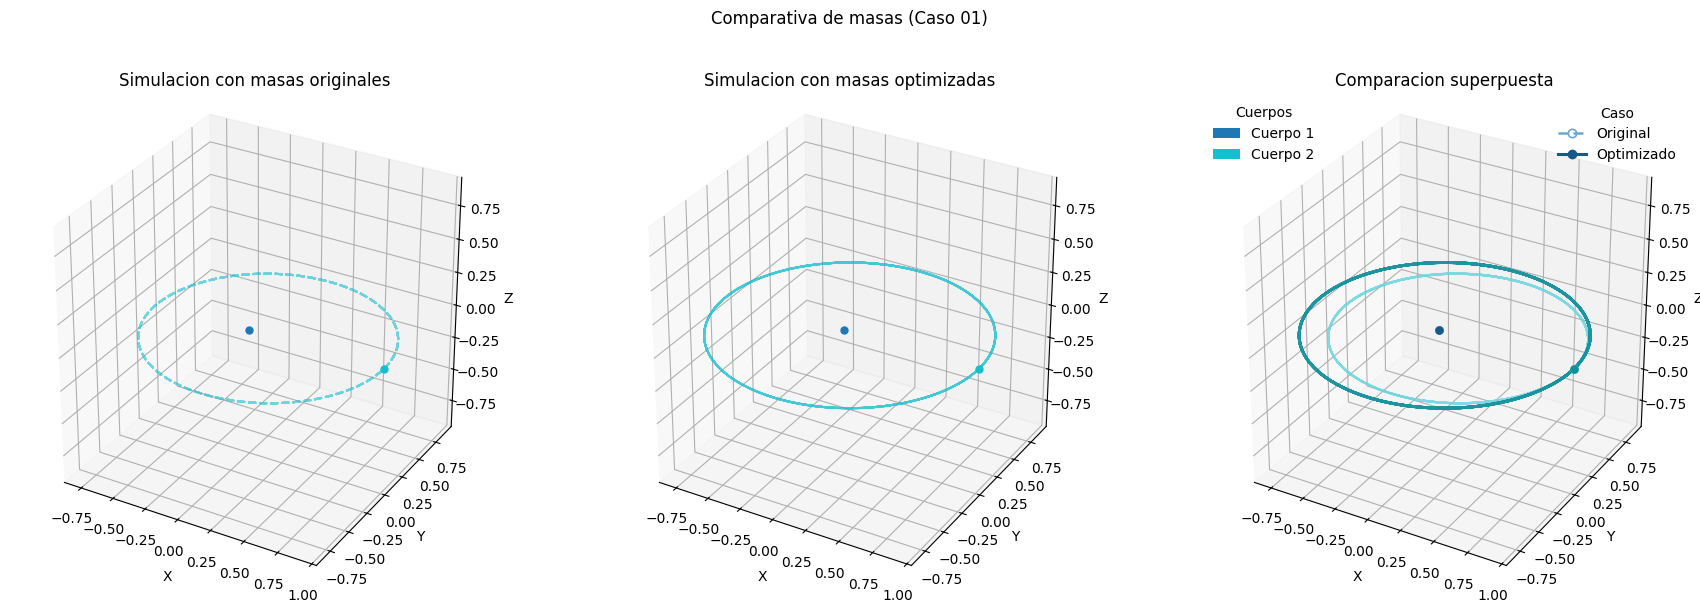
\includegraphics{img/resultados/caso03-comparativa_trayectoria.png}%
            }
            \\[-0.15cm]
            {\tiny Comparativa de trayectorias (original vs optimizada).}
        \end{column}
        \begin{column}{0.48\textwidth}
            \centering
            \adjustbox{max width=\linewidth, max height=0.7\textheight}{%
                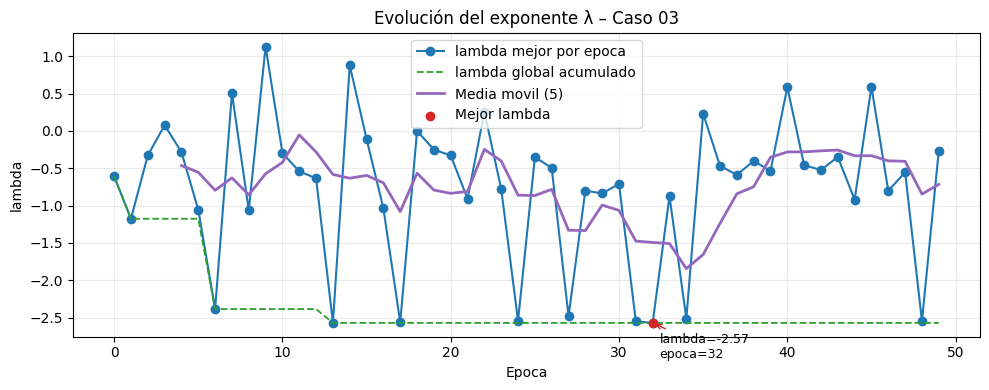
\includegraphics{img/resultados/caso03-evolucion_exponente.png}%
            }
            \\[-0.15cm]
            {\tiny Evolución del exponente de Lyapunov $\lambda$.}
        \end{column}
    \end{columns}
\end{frame}

